\chapter{A Unified Model for Multi-Modal Attention} 
\label{chapter-unified} 

The purpose of using EMMA is to help the multi-modal network (MMN) to handle failing modes, but also as a side effect, modes with different contributions and modes with different levels of noise. Chapter \ref{chapter-literature-review} discussed self-attention and crossmodal attention that are used to highlight information inside a specific mode, such as certain regions in an image or a set of frequencies in a sound. The difference between the two is that self-attention uses only the information of the mode itself as a context, whereas crossmodal attention leverages the information in all the modes. We claim to have all the ingredients to construct a complete multi-modal network. As a reminder, human's multi-modal attention consists of three different components: exogenous, endogenous and crossmodal attention. Attention is endogenous when we voluntary choose to attend to something whereas exogenous orients occurs when a person's attention is captured reflexively by the sudden onset of an unexpected event \citep{crossmodal}. Thus, an endogenous module could easily be constructed as a block of $M$ self-attentions. Moreover, EMMA can be considered to be equivalent to exogenous attention. 

\begin{figure}[hbt!]
\centering
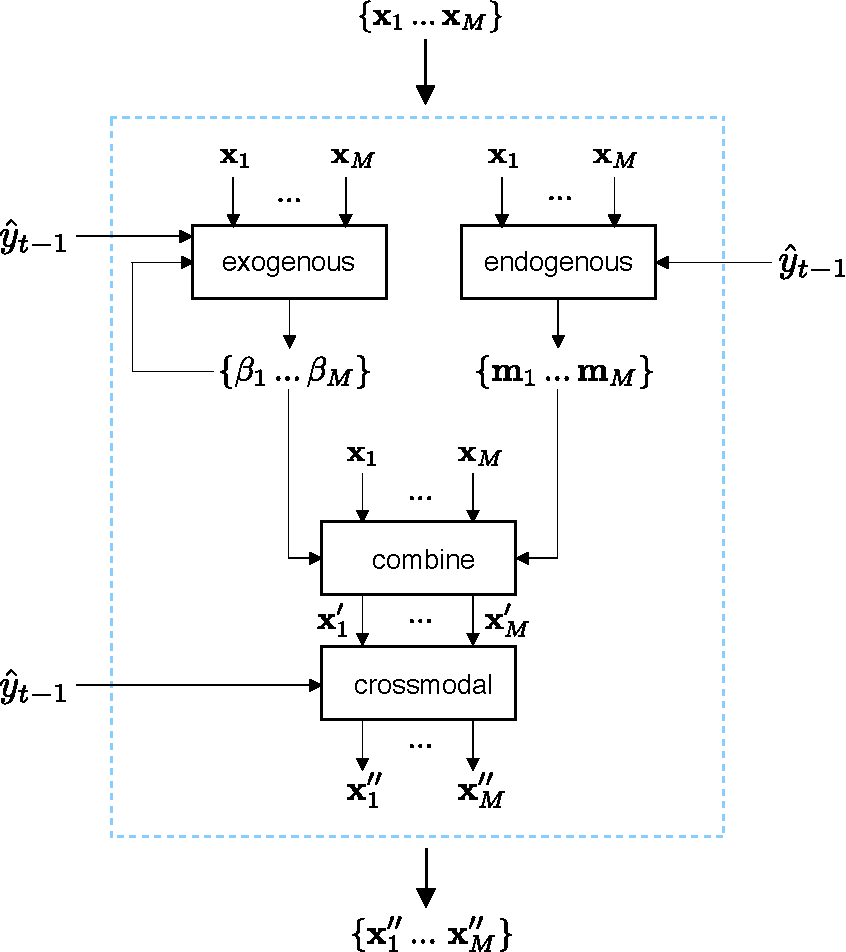
\includegraphics[scale=0.5]{figures/unified}
\caption{A possible architecture for a unified multi-modal attention}
\label{fig:complete-model}
\end{figure}

With this in mind, we present a unified model (see Figure \ref{fig:complete-model}) combining all the strengths of each type of attention. First, the attention masks of the exogenous model, $\beta_i$, and the attention masks of the endogenous module, $\mathbf{m}_i$, are combined as $\beta_i\mathbf{m}_i$. The resulting mask is then applied to the input sample, and is passed through the crossmodal module, which explores the relationships between the modes of the input. Finally, the processed input $\{\mathbf{x}'_1\,...\,\mathbf{x}'_M\}$ is forwarded to the MMN. In addition, the complete module can be further refined by inserting feedback loops from the predicted output to the separate modules as it is often done in the literature \citep{afouras, attention-need, bahdanau}. For example, in a self-driving system, the model could adapts its focus to different regions of the input image depending on the previously detected cars. To conclude, let us emphasize that the proposed architecture is only a generalization of attention networds such as \citep{afouras}, supplemented with an exogenous component.


